%!TEX root = ../main.tex
%%%%%%%%%%%%%%%%%%%%%%%%%%%%%%%%%%%%%%%%%
%
%LEZIONE 28/02/2017 - PRIMA SETTIMANA (1)
%
%%%%%%%%%%%%%%%%%%%%%%%%%%%%%%%%%%%%%%%%%
\chapter{Introduzione alla crittografia}

	In questo capitolo introduttivo daremo la definizione di crittosistema ed analizzeremo alcuni esempi classici di cifrari.
	Questo corso è incentrato sulla crittografia a chiave pubblica, la quale verrà introdotta nel successivo capitolo.
	Ciò che segue è quindi una breve introduzione alla crittografia classica che esula dagli scopi di questo corso.

	Classicamente la crittografia nasce con lo scopo di nascondere il contenuto di un messaggio.
	Recentemente i suoi usi sono stati ampliati:
	\begin{itemize}
		\item Autenticazione di un messaggio o di un interlocutore.
		\item Scambio di una chiave segreta.
		\item Firma digitale.
		\item Condivisione di un segreto
	\end{itemize}

	Tradizionalmente si utilizzano dei personaggi fittizi per illustrare la situazione: classicamente avremo \emph{Alice} che deve comunicare con \emph{Bob}; entrambi devono però tenere conto della presenza di un attaccante \emph{Eve} che può ascoltare la conversazione.

\section{Cifrari storici}

	Analizziamo di seguito due semplici cifrari usati in epoca antica:
	\begin{description}
		\item[Atbash] è un cifrario a sostituzione monoalfabetica in cui la prima lettera dell'alfabeto è sostituita con l'ultima, la seconda con la penultima e così via. Ad esempio:
			\[
			\text{ciao} \longrightarrow \text{YRZL}
			\]
		\item[Scitala] è uno dei più antichi metodi di crittografia per trasposizione conosciuti: il meccanismo di codifica permetteva, nel caso la scitala fosse stata intercettata dal nemico, di mantenere segreto il contenuto del messaggio e, nello stesso tempo, consentiva al ricevente di verificarne l'autenticità, in quanto solo chi era dotato di una bacchetta identica a quella utilizzata dal mittente per preparare la scitala, poteva decifrare e leggere il messaggio. Nella figura \autoref{fig:scitala} ve ne è una ricostruzione.
	\end{description}

	\begin{figure}[tb]
	\centering
		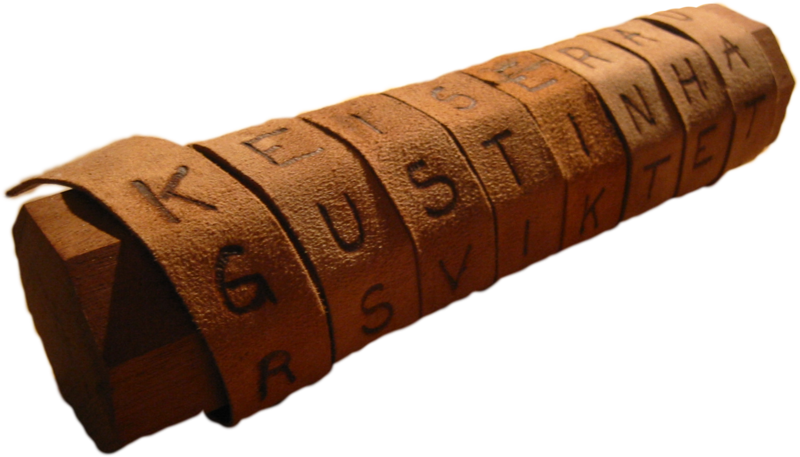
\includegraphics[width=0.5\textwidth]{Immagini/scitala.png}
		\caption{Una ricostruzione di scitala.}
		\label{fig:scitala}
	\end{figure}

\section{Crittosistemi}

	\begin{defn}{Crittosistema}{crittosistema}\index{Crittosistema}
	Un \emph{crittosistema} è una quintupla \((P,C,K,E,D)\), dove
	\begin{itemize}
		\item \(P\) è un insieme finito di testi in chiaro o \emph{plaintext}.
		\item \(C\) è un insieme finito di testi cifrati o \emph{ciphertext}.
		\item \(K\) è un insieme finito di chiavi o \emph{spazio delle chiavi}
		\item Per ogni \(k\in K\) c'è una funzione di cifratura \(e_k\in E\), con \(e_k\colon P \to C\), e una funzione di decifratura \(d_k\in D\), con \(d_k\colon C \to P\), tali che
			\[
			d_k\big(e_k(x)\big) = x
			\]
		per ogni \(x\in P\).
	\end{itemize}
	\end{defn}
	
	\begin{oss}
	Chiaramente se \(x,y\in P\) con \(x\neq y\), si deve avere che, per ogni chiave \(k\),
		\[
		e_k(x) \neq e_k(y).
		\]
	Ovvero le funzioni di \(E\) devono essere iniettve.
	\end{oss}

	\begin{ese}[Cifrario additivo]
	Posti \(P,C,K=\Z_{26}\), fissiamo \(k\in[0,25]\) e definiamo
		\[
		e_k(x) = x+k \pmod{26} \qquad\text{e}\qquad d_k(y) = y-k \pmod{26}.
		\]
	Quando \(k=3\) tale cifrario prende il nome di \emph{cifrario di Cesare}.

	Chiaramente possiamo riportarci all'alfabeto identificando \(\Z_{26}\) con le lettere.
	\end{ese}

	Affinché un crittosistema possa essere considerato efficiente e sicuro, si devono soddisfare due proprietà basilari:
	\begin{itemize}
		\item Dev'essere possibile calcolare ogni \(e_k\) e \(d_k\) in modo computazionalmente efficiente.
		\item \emph{Eve} non deve essere in grado di risalire al testo in chiaro (o peggio, alla chiave) dal testo cifrato.
	\end{itemize}
	Nell'esempio dei cifrari additivi descritto poc'anzi, si hanno solamente 26 possibili chiavi.
	Ciò rende il crittosistema incredibilmente insicuro e attaccabile persino a mano.

	Osserviamo che per definizione, \(P\) e \(C\) sono insiemi finiti e le funzioni di cifratura devono essere iniettive.
	Se in un crittosistema si ha \(P=C\), sappiamo che una funzione \(f\colon P \to C = P\) è iniettiva se e soltanto se è suriettiva.
	Quindi tutte le funzioni di cifratura sono biiettive. In tal caso \(E\) sono le permutazioni di \(P\).
	Se \(P\) ha \(n\) elementi avremo che \(E=S_n\) ha \(n!\) elementi.

	\begin{ese}[Cifrari a sostituzioni]
	Posti \(P=C=\Z_{26}\) e \(K=S_{26}\), per ogni \(\p\in K\) avremo
		\[
		e_\p(x) = \p(x) \qquad\text{e}\qquad d_\p(y) = \p^{-1}(y).
		\]
	In questo caso il numero di chiavi è pari a \(26! \approx 4\cdot 10^{26}\).
	Nonostante questo numero sia molto grande, ciò non basta a garantire la sicurezza di questo crittosistema.
	Questo metodo di cifratura lascia infatti inalterate le regolarità della lingua che permettono una facile decifratura.
	\end{ese}

\section{Crittoanalisi}

	Storicamente con il termine \emph{crittonalisi}, si fa riferimento ai metodi di attacco contro un generico crittosistema.

	\begin{defn}{Principio di Kerckhoffs}{principioKerckhoffs}
	Il principio di Kerckhoffs afferma che la sicurezza di un crittosistema non deve dipendere dal tenere celato il crittoalgoritmo ma solo dal tenere celata la chiave.
	\end{defn}

	In altre parole, il principio di Kerckhoffs afferma che nella costruzione di un crittosistema si deve lavorare affinché il sistema rimanga sicuro anche nell'ipotesi che l'attaccante conosca l'algoritmo di crittazione. Tale principio ha diversi vantaggi:
	\begin{itemize}
		\item \'E più facile tenere segreta la chiave.
		\item Se la sicurezza si basa sulla chiave, e la chiave viene scoperta, basta cambiare chiave.
		\item Si può usare lo stesso crittosistema per far comunicare diverse coppie di persone
		\item Un sistema che viene molto studiato (e attaccato) è più sicuro.
		\item Meglio che le debolezze, se ci sono, vengano scoperte e rese pubbliche.
		\item Se l'algoritmo è pubblico, non c’`e rischio di reverse engineering.
		\item Si possono stabilire standard.
	\end{itemize}
	Oggi il principio di Kerckhoffs viene inteso in maniera più forte: l'algoritmo deve essere pubblico.

	Tornando alla crittoanalisi, elenchiamo alcuni tipi di attacco:
	\begin{description}
		\item[Ciphertext only attack] L'attaccante conosce una stringa \(y\) di testo cifrato. Cerca di risalire al testo in chiaro o alla chiave.
		\item[Known plaintext attack] L'attaccante conosce una stringa \(x\) di testo in chiaro e il corrispondente testo cifrato \(y\). Cerca di risalire alla chiave o di decrittare altri testi cifrati.
		\item[Chosen plaintext attack] L'attaccante ha la possibilità di scegliere un testo in chiaro \(x\) e di ottenere il corrispondente testo cifrato \(y\). Cerca di risalire alla chiave o di decrittare altri testi cifrati.
		\item[Chosen ciphertext attack] L'attaccante ha la possibilità di scegliere un testo cifrato \(y\) e di ottenere il corrispondente testo in chiaro \(x\). Cerca di risalire alla chiave.
	\end{description}